\documentclass[aspectratio=169,11pt]{beamer}
\usetheme{default}
\usepackage{amsmath,amssymb,booktabs,tikz,graphicx,url}
\definecolor{navy}{HTML}{17324D}\definecolor{teal}{HTML}{0B7A75}\definecolor{gold}{HTML}{E6A23C}\definecolor{mist}{HTML}{F2F6F8}
\setbeamercolor{normal text}{fg=navy,bg=white}\setbeamercolor{frametitle}{fg=white,bg=navy}\setbeamercolor{structure}{fg=teal}
\setbeamertemplate{navigation symbols}{}\setbeamertemplate{footline}{\hfill\insertframenumber/\inserttotalframenumber\hspace{1em}\vspace{.6em}}
\newcommand{\takeaway}[1]{\vfill\colorbox{mist}{\parbox{.94\linewidth}{\textbf{Takeaway:} #1}}}
\title{Agentic Delegation and the Language Frontier}\subtitle{A model, GitHub evidence, and a Lean audit}
\author{Course replication: ai-03-quispe}\date{Quispe \& Xu (2026), arXiv:2605.25438v2}
\begin{document}
\begin{frame}\titlepage\vfill\centering\small\url{https://github.com/davidolano03/ai-03-quispe}\end{frame}

\begin{frame}{First check: the requested citation was stale}
\begin{columns}[T]\column{.47\textwidth}\textbf{Prompted title}\par\medskip
``Coding Beyond Your Training: Claude Code and the Technological Frontier of Software Developers''
\column{.47\textwidth}\textbf{Verified arXiv v2}\par\medskip
``Agentic Delegation and the Language Frontier of Software Developers: A Model and Evidence from Claude Code on GitHub''\\[.6em]Alexander Quispe \& Kevin Xu
\end{columns}\takeaway{The title, author list, version date, and sample size were checked before analysis.}\end{frame}

\begin{frame}{Question and contribution}
\Large Can an agentic coding tool move developers beyond their prior language frontier?\normalsize
\begin{enumerate}\item A delegation model of extensive-margin entry.\item GitHub evidence around voluntary Claude Code adoption.\item Heterogeneity predictions for specialists and lower-ability developers.\item A formal audit of all five propositions.\end{enumerate}
\takeaway{The novel mechanism is entry into unfamiliar technical domains, not only faster coding.}\end{frame}

\begin{frame}{The agent's economic role}
For language $\ell$, solo and delegated project values are $V^0_\ell$ and $V^A_\ell$.
\[\text{before}=\mathbf 1\{V^0_\ell\ge0\},\qquad \text{with agent}=\mathbf 1\{\max(V^0_\ell,V^A_\ell)\ge0\}.\]
New activation occurs when $V^0_\ell<0\le V^A_\ell$.
\begin{center}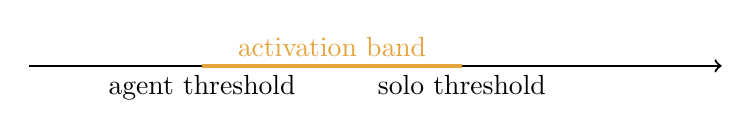
\begin{tikzpicture}[x=1.1cm]\draw[->,thick] (0,0)--(8,0); \draw[gold,very thick] (2,0)--(5,0);\node[below] at (2,0){agent threshold};\node[below] at (5,0){solo threshold};\node[above,gold] at (3.5,0){activation band};\end{tikzpicture}\end{center}
\takeaway{Delegation lowers the threshold for attempting an unfamiliar language.}\end{frame}

\begin{frame}{Five propositions, one logical chain}\small
\begin{tabular}{p{.08\linewidth}p{.82\linewidth}}\toprule
P1 & Taking the better of solo and delegated value weakly expands the frontier.\\
P2 & Expansion equals probability mass in the activation band.\\
P3 & Repeated activation creates a growing cumulative gap with diminishing increments.\\
P4 & Effects are larger with more unfamiliar candidates and higher activation probability.\\
P5 & Lower repository-entry costs weakly increase repository breadth; strictness needs positive band mass.\\\bottomrule
\end{tabular}\takeaway{Weak expansion follows from option value; strict expansion always needs positive mass.}\end{frame}

\begin{frame}{Data and identification}
\begin{columns}[T]\column{.45\textwidth}\textbf{Panel}\begin{itemize}\item 5,346 developers\item 149,688 developer-months\item Jan. 2024--Apr. 2026\item 3.2m commits; 57m files\end{itemize}
\column{.49\textwidth}\textbf{Design}\begin{itemize}\item First Claude-coauthored commit marks adoption\item Early vs. not-yet-treated adopters\item Callaway--Sant'Anna doubly robust staggered DiD\item One-month anticipation window\end{itemize}\end{columns}
\takeaway{The comparison is carefully structured, but adoption remains voluntary.}\end{frame}

\begin{frame}{Main event-study magnitudes}\centering
\begin{tabular}{lrrr}\toprule & Adoption & $t+1$ & $t+2$\\\midrule
Languages & $+2.528$ & $+1.227$ & $+0.693$\\New languages & $+1.193$ & $+0.126$ & $-0.018$\\Language entropy & $+0.382$ & $+0.189$ & $+0.102$\\\bottomrule\end{tabular}
\vspace{1em}\par Pre-period means: 0.90 languages and 0.31 new languages per developer-month.
\takeaway{A sharp adoption spike leaves persistent breadth, while the flow of new entry quickly fades.}\end{frame}

\begin{frame}{Is this only Claude writing the new-language code?}
\begin{itemize}\item Excluding the language of the first Claude commit: $+1.58$ languages and $+0.807$ new languages at adoption.\item Removing all Claude-coauthored commits: $+1.663$ languages and $+0.724$ new languages.\item Roughly two-thirds of diversification remains after removing detectable agent-authored commits.\item Per-commit diversification is concentrated at adoption; persistence is partly higher activity volume.\end{itemize}
\takeaway{The pattern is broader than mechanical counting, but it is not a randomized treatment effect.}\end{frame}

\begin{frame}{Where I distrusted the paper: Proposition 3}
For $p_1=0$, the cumulative gap for one unfamiliar language is
\[G(t)=1-(1-p_2)^{t+1},\qquad \Delta G(t)=p_2(1-p_2)^{t+1}.\]
The paper permits $p_2=1$, but then $G(t)=1$ for all $t$: strict growth and strict concavity fail. The sum is also not strict when the unfamiliar set is empty.
\IfFileExists{hand/derivation.jpg}{\begin{center}\includegraphics[height=2.2cm]{hand/derivation.jpg}\end{center}}{\begin{center}\fbox{\parbox{.72\linewidth}{\centering Add authentic photo: \texttt{hand/derivation.jpg}\\Exact steps: \texttt{hand/DERIVATION.md}.}}\end{center}}
\takeaway{Verdict: weak result verified; strict result requires a nonempty set and $0<p_2<1$.}\end{frame}

\begin{frame}[fragile]{From the paper to Lean}
\textbf{Original equation}\[G(t)=\sum_{\ell\in U}\big[(1-p_{1\ell})^{t+1}-(1-p_{2\ell})^{t+1}\big].\]
\textbf{Lean statement/proof fragment}
\begin{verbatim}
intro hNonempty hClosedFrontier horizon
apply Finset.sum_lt_sum
  (fun l hl => (hTermIncreases l hl).le)
rcases hNonempty with <l, hl>
exact <l, hl, hTermIncreases l hl>
\end{verbatim}
\textbf{My reading:} strictness needs a witness language plus an interior hazard. All five proof endpoints compile; no \texttt{sorry} or \texttt{admit} is used.
\end{frame}

\begin{frame}{Assumptions made explicit}
\begin{enumerate}\item \textbf{Foothold:} augmentation helps only after a familiar-language foothold; otherwise delegation drives entry.\item \textbf{Verification technology:} verification costs change with agent quality and ability in the directions used by the comparative statics.\item \textbf{Comparable candidates:} unfamiliar languages share an activation probability in the parsimonious heterogeneity result.\end{enumerate}
\takeaway{Lean checks implication structure, not whether behavioral assumptions are empirically true.}\end{frame}

\begin{frame}{Comparison with Aouad--Lykouris--Zhong}\small
\begin{tabular}{p{.25\linewidth}p{.32\linewidth}p{.32\linewidth}}\toprule & Quispe--Xu & Aouad--Lykouris--Zhong\\\midrule
AI role & Information, delegation, verification & Substitutable productive input\\Margin & Domain/language entry & Task allocation and human capital\\Risk & Selection into new projects & Deskilling / investment displacement\\Key choice & Outside option plus threshold band & Dynamic substitution technology\\\bottomrule\end{tabular}
\takeaway{Modeling AI as delegation generates frontier expansion; modeling it as an input foregrounds deskilling.}\end{frame}

\begin{frame}{Three critiques}
\begin{enumerate}\item The entry threshold may also represent a generic productivity shock; the model does not uniquely identify delegation.\item The design cannot cleanly separate causal expansion from selection into projects that both require new languages and prompt Claude adoption.\item Several strict propositions omit endpoint conditions; positive mass, nonempty sets, and interior hazards must be stated.\end{enumerate}
\takeaway{The descriptive pattern is strong; the mechanism and causal interpretation remain less settled.}\end{frame}

\begin{frame}{Conclusion}\Large Agentic AI appears to broaden what developers attempt.\normalsize
\begin{itemize}\item Adoption coincides with a large, partly persistent expansion in language breadth.\item Delegation offers a coherent extensive-margin mechanism.\item Robustness checks reduce, but do not eliminate, selection concerns.\item Formalization validates the weak results and repairs the strict dynamic claim.\end{itemize}
\vfill\centering\textbf{Repository:} \url{https://github.com/davidolano03/ai-03-quispe}\end{frame}
\end{document}
